\documentclass[aspectratio=169,11pt]{beamer}

\setbeamertemplate{navigation symbols}{}
\useinnertheme[shadow=true]{rounded}
\useoutertheme{infolines}
\setbeamertemplate{footline}[frame number]
\definecolor{purpleheart}{RGB}{078, 042, 132}
\setbeamercolor{title}{fg=white,bg=purpleheart}
\setbeamercolor{palette tertiary}{fg=white,bg=purpleheart}
\setbeamercolor{frametitle}{fg=purpleheart,bg=gray!0}
\setbeamercolor{button}{bg=purpleheart}
\setbeamertemplate{itemize item}[circle]
\setbeamertemplate{enumerate item}[default]
\setbeamertemplate{itemize subitem}[triangle]
\setbeamercolor{itemize item}{fg=purpleheart}
\setbeamercolor{itemize subitem}{fg=purpleheart}
\setbeamercolor{enumerate item}{fg=purpleheart}
\setbeamercolor{part title}{fg=white,bg=purpleheart}
\setbeamertemplate{section page}
{
    \begin{centering}
    \begin{beamercolorbox}[wd=\paperwidth,sep=12pt,center]{part title}
    \usebeamerfont{section title}\insertsection\par
    \end{beamercolorbox}
    \end{centering}
}
\setbeamertemplate{title page}[default][rounded=true]
\usepackage{graphicx}
\usepackage{booktabs}
\usepackage{amsthm}
\usepackage{amssymb}
\usepackage{amsmath} 
\usepackage{bbm}
\usepackage{array}
\usepackage{hyperref}
\usepackage{appendixnumberbeamer}
\usepackage{verbatim}
\newtheorem{assumption}{Assumption}
\newcommand{\beginbackup}{
   \newcounter{framenumbervorappendix}
   \setcounter{framenumbervorappendix}{\value{framenumber}}
   \setbeamertemplate{footline}
   {
     \leavevmode%
     \hline
     box{%
       \begin{beamercolorbox}[wd=\paperwidth,ht=2.25ex,dp=1ex,right]{footlinecolor}%
%         \insertframenumber  \hspace*{2ex} 
       \end{beamercolorbox}}%
     \vskip0pt%
   }
 }
\newcommand{\backupend}{
   \addtocounter{framenumbervorappendix}{-\value{framenumber}}
   \addtocounter{framenumber}{\value{framenumbervorappendix}} 
}

\begin{document}
\title[Beamer]{A Beamer Template}
\author[Name]{\textbf{Your Name} \\Your Institution}

\begin{frame}[plain,noframenumbering]
\titlepage
\end{frame}

\section{Introduction}
\begin{frame}[fragile]{Motivation}
\begin{itemize}
    \item Use \verb|\pause| to make items appear sequentially 
    \begin{itemize}
        \item Sub Bullet 1
        \item Sub Bullet 2
        \pause
        \item Sub Bullet 3
    \end{itemize}
    \pause
    \item Bullet 2
    \begin{itemize}
        \item Sub Bullet 1 
        \item Sub Bullet 2
    \end{itemize}
    \pause 
    \item Bullet 3
\end{itemize}
\end{frame}

\begin{frame}{Preview}
    \begin{itemize}
        \item Show the first bullet point and the first figure.
        \item<2-> Add one bullet point and show the second figure in the same place.
    \end{itemize}
    \begin{figure}
        \centering
        \includegraphics<1>[height=0.7\textheight]{fig/scatter.pdf}%
        \includegraphics<2->[height=0.7\textheight]{fig/hist.pdf}%
    \end{figure}    
\end{frame}

\begin{frame}{Vertical Style}
    \begin{columns}[T] % align columns
        \begin{column}{.55\textwidth}
            \begin{center}
                {
                \includegraphics<1>[width=\textwidth]{fig/scatter.pdf}%
                \includegraphics<2>[width=\textwidth]{fig/hist.pdf}%
                }
            \end{center}
        \end{column}
        \begin{column}{.45\textwidth}
            \begin{itemize}
                \item<1> Result 1
                \item<2> Result 2 (no Result 1)
            \end{itemize}
        \end{column}
    \end{columns}    
\end{frame}

\begin{frame}{Outline for Today}
    \begin{columns}[c] % align columns
        \begin{column}{.45\textwidth}
            \begin{enumerate}
                \item Data
                \item Empirical Strategy
                \item Results
                \item Conclusion
            \end{enumerate}
        \end{column}
        \begin{column}{.45\textwidth}
            \begin{center}
                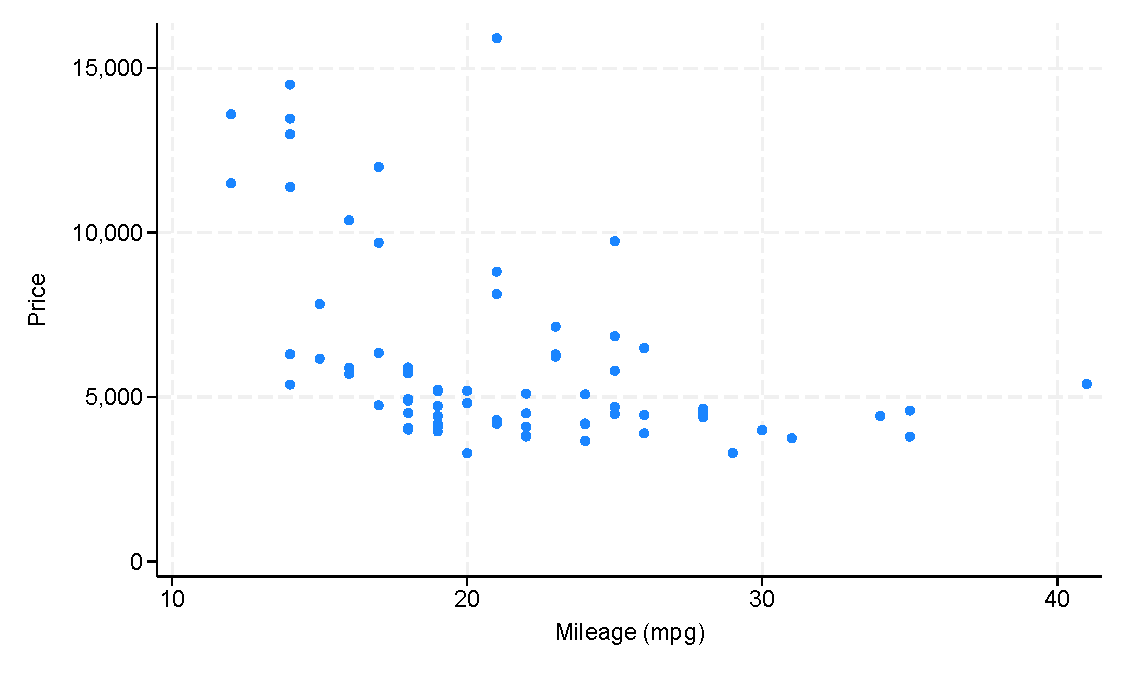
\includegraphics[width=\textwidth]{fig/scatter.pdf}%
            \end{center}
        \end{column}
    \end{columns}    
\end{frame}

\section{Data}
\begin{frame}[plain,noframenumbering]
\sectionpage
\end{frame}

\begin{frame}[label=data]{Data Source}
    \begin{itemize}
        \item Go to Data Appendix. \hyperlink{data_appendix}{\beamergotobutton{Data Appendix}}
    \end{itemize}
    
\end{frame}


\section{Empirical Strategy}
\begin{frame}[plain,noframenumbering]
\sectionpage
\end{frame}

\begin{frame}{OLS}
    \begin{equation}
        y_{it} = \alpha + \textcolor{red}{\beta X_{it}} + \varepsilon_{it}
    \end{equation}
    \begin{itemize}
        \item $y_{it}$
        \item $X_{it}$
    \end{itemize}
\end{frame}

\section{Results}
\begin{frame}[plain,noframenumbering]
\sectionpage
\end{frame}

\begin{frame}{Single Plot}
    \begin{figure}
        \centering
        \includegraphics[width=0.8\textwidth]{fig/single.pdf}
    \end{figure}
\end{frame}

\begin{frame}{Two Plots}
    \begin{figure}
        \includegraphics[width=0.495\textwidth, height=0.7\textheight]{fig/single.pdf}
        \hfill
        \includegraphics[width=0.495\textwidth, height=0.7\textheight]{fig/single.pdf}
    \end{figure}
\end{frame}

\begin{frame}{Show Table Rows Sequentially}
    \centerline{
        \scalebox{0.95}{
            \begin{tabular}{lcccc }
                \toprule
                Competitor Name & Swim & Cycle & Run & Total \\
                \midrule
                John T & 13:04 & 24:15 & 18:34 & 55:53 \onslide<2-> \\ 
                Norman P & 8:00 & 22:45 & 23:02 & 53:47 \onslide<3->\\
                Alex K & 14:00 & 28:00 & n/a & n/a \onslide<4->\\
                Sarah H & 9:22 & 21:10 & 24:03 & 54:35 \\
                \bottomrule
            \end{tabular}
        }
    }
\end{frame}

\begin{frame}{Show Table Columns Sequentially}
    \centerline{
        \scalebox{0.95}{
            \begin{tabular}{l<{\onslide<1->}c<{\onslide<2->}c<{\onslide<3->}c<{\onslide}} 
            \toprule
            Dependent variable & \multicolumn{3}{c}{$\mathbbm{1}$(Y)}\\ 
            \midrule
            & (1) & (2) & (3)\\
            \midrule
            X & 0.102*** & 0.100*** & \textcolor{red}{0.064***}\\
            & (0.009) & (0.009) & \textcolor{red}{(0.008)} \\
            \midrule
            Observations & 1,000 & 1,000 & 1,000 \\
            Time FEs &  & \checkmark & \checkmark \\
            County FEs &  &  & \checkmark \\
            \bottomrule
            \end{tabular}
        }
    }
\end{frame}

\section{Conclusion}
\begin{frame}{Conclusion}
\end{frame}

\section{Thanks!}
\begin{frame}[plain,noframenumbering]
\sectionpage
\end{frame}

\section{Appendix}
\appendix
\begin{frame}[label=data_appendix]{Backup Slides}
\begin{itemize}
    \item Appendix starts from here.
    \item Restart the numbering.
    \item Go back to Data. \hyperlink{data}{\beamergotobutton{Back}}   
\end{itemize}
\end{frame}

\begin{frame}{Robustness Checks}

\end{frame}

\end{document}